% ==============================================================================
% WEEK 6
% ==============================================================================
\section{Week 6 -- 23.03.26 - Residues}

\begin{definition}[Definition: Residue]
The coefficient $c_{-1}$ of the term $(z - z_0)^{-1}$ in the Laurent series for $f$ at $z_0$ is called the \textbf{residue} of $f$ at $z_0$.
\[ \Res_{z_0}(f) := c_{-1} \]

In view of the definition of the coefficients of the Laurent series:
\[ c_{-1} = \frac{1}{2\pi i} \int_\gamma f(z) dz \]
for any curve $\gamma$ which is closed, simple, counter-clockwise oriented, contains $z_0$ in its interior, and $f$ is holomorphic on $\interior(\gamma) \setminus \{z_0\}$.
\end{definition}

\begin{example}[Trivial \& Basic Examples]
\textbf{Trivial example:} If $f$ is holomorphic on a set $D$ containing $z_0$, then $\Res_{z_0}(f) = 0$ (Cauchy's theorem).

\textbf{Basic example:} $\Res_0\left(\frac{1}{z}\right) = 1$ (since $f(z) = \frac{1}{z}$ already is expressed as its Laurent series at $z_0 = 0$).
\end{example}

\begin{remark}[Note: Extracting the Residue for a Pole of Order $m$]
Suppose that $f(z)$ has a pole of order $m$ at $z_0$:
\[ f(z) = c_{-m}(z - z_0)^{-m} + \dots + c_{-1}(z - z_0)^{-1} + c_0 + \dots \]
Then: 
\begin{align*}
g(z) &= (z - z_0)^m f(z) \\
&= c_{-m} + c_{-m+1}(z - z_0) + \dots + c_{-1}(z - z_0)^{m-1} + \dots
\end{align*}
is the Taylor series of the regular function $g$ at $z_0$.

Thus: We can extract the residue using the formula for the Taylor coefficients:
\[ c_{-1} = \frac{1}{(m-1)!} \frac{d^{m-1}}{dz^{m-1}} (g(z))\bigg|_{z=z_0} = \lim_{z \to z_0} \frac{1}{(m-1)!} \frac{d^{m-1}}{dz^{m-1}} \left((z - z_0)^m f(z)\right) \]

The above formula is useful if we already know that $f$ has a pole of order $m$ at $z_0$.

\vspace{0.3cm}
\textbf{Most useful: When $m = 1$.} In that case:
\[ \Res_{z_0}(f) = \lim_{z \to z_0} \left((z - z_0) \cdot f(z)\right) \]
\end{remark}

\begin{example}[Example]
$f(z) = \frac{1}{\sin(z)}$, $z_0 = 0$.

Note:
\[ f(z) = \frac{1}{z - \frac{z^3}{3!} + \dots} = \frac{1}{z} \cdot \frac{1}{1 - \frac{z^2}{3!} + \dots} \]
So $f$ has a pole of order 1 at $z_0 = 0$. (It would also follow from our more general discussion last time for functions of the form $\frac{p(z)}{q(z)}$).

So: 
\begin{align*}
\Res_0(f) &= \lim_{z \to 0} (z \cdot f(z)) \\
&= \lim_{z \to 0} \frac{z}{\sin(z)} \\
&= \lim_{z \to 0} \frac{z}{z - \frac{z^3}{3!} + \dots} \\
&= \lim_{z \to 0} \frac{1}{1 - \frac{z^2}{3!} + \dots} = 1
\end{align*}
\end{example}

\subsection{Residue Theorem and Applications}

\textbf{Recall:} If $f$ is holomorphic ``around'' $z_0$, but with a possible singularity at $z_0$:
\[ \int_\gamma f(z) dz = 2\pi i \Res_{z_0}(f) \]
if $\gamma$ is simple, closed, counter-clockwise oriented, contains $z_0$ and no other singularity of $f$ (so $f$ is holomorphic on the set $\interior(\gamma) \setminus \{z_0\}$).

\vspace{0.3cm}

\begin{theorem}[Theorem: Residue Theorem]
Suppose that $D \subseteq \mathbb{C}$ is open and simply connected and let $\gamma$ be a simple, closed curve in $D$ which is counter-clockwise oriented. Let $z_1, z_2, \dots, z_m \in \interior(\gamma)$. 

If $f: D \setminus \{z_1, z_2, \dots, z_m\} \longrightarrow \mathbb{C}$ is holomorphic, then
\[ \int_\gamma f(z) dz = 2\pi i \left(\Res_{z_1}(f) + \dots + \Res_{z_m}(f)\right) \]

\textit{Remark:} In order to compute $\int_\gamma f(z) dz$, it therefore suffices to compute the residues of $f$ at the singular points in the interior of $\gamma$.
\end{theorem}

\begin{proofbox}[Sketch of the proof (by picture)]
Assume (without loss of generality) that we only have two singular points: $z_1$ and $z_2$. By the extension of Cauchy's theorem, integrating over a deformed contour that isolates the singularities gives zero. When the ``bridge'' is too narrow: The integral over the straight path components cancels out, leaving us with the two integrals over the smaller loops $\gamma_1$ and $\gamma_2$ around $z_1$ and $z_2$, respectively:
\[ \int_\gamma f(z) dz = \int_{\gamma_1} f(z) dz + \int_{\gamma_2} f(z) dz = 2\pi i \Res_{z_1}(f) + 2\pi i \Res_{z_2}(f) \]
\end{proofbox}

\subsubsection{Examples}

\begin{example}[Example 1]
Consider $f(z) = \frac{1}{z}$, let $\gamma$ be a simple, closed, counter-clockwise oriented curve in $\mathbb{C}$. Compute $\int_\gamma f(z) dz$.

\begin{itemize}
    \item \textbf{Case 1:} $0 \in \interior(\gamma)$. Then $\int_\gamma f(z) dz = 2\pi i \Res_0\left(\frac{1}{z}\right) = 2\pi i$.
    \item \textbf{Case 2:} $0 \notin \overline{\interior(\gamma)} = \interior(\gamma) \cup \gamma$. Then $\int_\gamma f(z) dz = 0$.
    \item \textbf{Case 3:} $0 \in \gamma$. In this case, $\int_\gamma f(z) dz$ is not well-defined.
\end{itemize}

\textit{Note:} 
\begin{itemize}
    \item $\interior(\gamma)$: The open set enclosed by $\gamma$ (so it doesn't contain $\gamma$).
    \item $\overline{\interior(\gamma)} = \interior(\gamma) \cup \gamma$: The closed set enclosed by $\gamma$ (so it contains the curve $\gamma$).
\end{itemize}
\end{example}

\begin{example}[Example 2]
Let $f: \mathbb{C} \setminus \{0, -1\} \longrightarrow \mathbb{C}$, $f(z) = \frac{1}{z \cdot (z+1)}$.

We have two poles of order 1 at $z_1 = 0$ and $z_2 = -1$.
\begin{align*}
\Res_0(f) &= \lim_{z \to 0} (z \cdot f(z)) = \lim_{z \to 0} \frac{1}{z+1} = 1 \\
\Res_{-1}(f) &= \lim_{z \to -1} ((z+1)f(z)) = \lim_{z \to -1} \frac{1}{z} = -1
\end{align*}

Let $\gamma$ be a simple, closed, counter-clockwise oriented curve. Compute $\int_\gamma f(z) dz = ?$
\begin{itemize}
    \item \textbf{Case A:} $0, -1 \notin \overline{\interior(\gamma)} \implies \int_\gamma f(z) dz = 0$.
    \item \textbf{Case B:} $0 \in \interior(\gamma), -1 \notin \overline{\interior(\gamma)} \implies \int_\gamma f(z) dz = 2\pi i \Res_0(f) = 2\pi i$.
    \item \textbf{Case C:} $0 \notin \overline{\interior(\gamma)}, -1 \in \interior(\gamma) \implies \int_\gamma f(z) dz = 2\pi i \Res_{-1}(f) = -2\pi i$.
    \item \textbf{Case D:} $0, -1 \in \interior(\gamma) \implies \int_\gamma f(z) dz = 2\pi i (\Res_0(f) + \Res_{-1}(f)) = 2\pi i (1 + (-1)) = 0$.
    \item \textbf{Case E:} $0 \in \gamma \lor -1 \in \gamma$. In this case, the integral is not well-defined.
\end{itemize}
\end{example}

\begin{example}[Example 3]
$f: \mathbb{C} \setminus \{0, 1\} \longrightarrow \mathbb{C}$, $f(z) = \frac{1}{z^2} + \frac{2}{z} + \frac{3}{z-1}$.

Pole of order 2 at 0, pole of order 1 at 1.
\begin{align*}
\Res_1(f) &= \lim_{z \to 1} ((z-1)f(z)) = \lim_{z \to 1} \left(\frac{z-1}{z^2} + \frac{2(z-1)}{z} + 3\right) = 3 \\
\Res_0(f) &= \lim_{z \to 0} \left(\frac{1}{1!} \frac{d}{dz}(z^2 f(z))\right) = \lim_{z \to 0} \left(\frac{d}{dz} \left(1 + 2z + \frac{3z^2}{z-1}\right)\right) \\
&= \lim_{z \to 0} \left(2 + \frac{6z}{z-1} - \frac{3z^2}{(z-1)^2}\right) = 2
\end{align*}
(\textit{I could have also deduced that by noting that $f(z) = \frac{1}{z^2} + \frac{2}{z} + \frac{3}{z-1}$, so from the singular part at $z=0$ we can trivially read off $c_{-1} = 2$}).

If $\gamma(t) = 10e^{it}, t \in [0, 2\pi]$:
$\interior(\gamma)$ contains both poles:
\[ \int_\gamma f(z) dz = 2\pi i (\Res_0(f) + \Res_1(f)) = 10\pi i \]
\end{example}

\begin{example}[Examples 4 \& 5]
\textbf{Example 4:} $\exp\left(\frac{1}{z}\right) = 1 + z^{-1} + \frac{z^{-2}}{2!} + \dots$ \\
$\Res_0\left(\exp\left(\frac{1}{z}\right)\right) = c_{-1} = 1.$

\vspace{0.2cm}
\textbf{Example 5:} $\exp\left(\frac{1}{z^2}\right) = 1 + z^{-2} + \frac{z^{-4}}{2!} + \dots$ \\
$\Res_0\left(\exp\left(\frac{1}{z^2}\right)\right) = 0.$
\end{example}

\subsection{Applications}

The residue theorem allows us to easily compute integrals over simple closed curves. Sometimes, we can write integrals over the real line as limits of integrals over closed curves in $\mathbb{C}$.

\begin{example}[Application Example: Integral over the Real Line]
\textbf{Compute:} $\int_{-\infty}^{+\infty} \frac{1}{1+x^2} dx$

Set $f(z) = \frac{1}{z^2+1}$. For any $R > 1$, consider the segment:
\[ L_R: [-R, R] \longrightarrow \mathbb{C}, \quad t \longmapsto t \quad (\text{segment on the real axis}) \]
and the half circle:
\[ C_R: [0, \pi] \longrightarrow \mathbb{C}, \quad t \longmapsto R e^{it} \]

\begin{center}
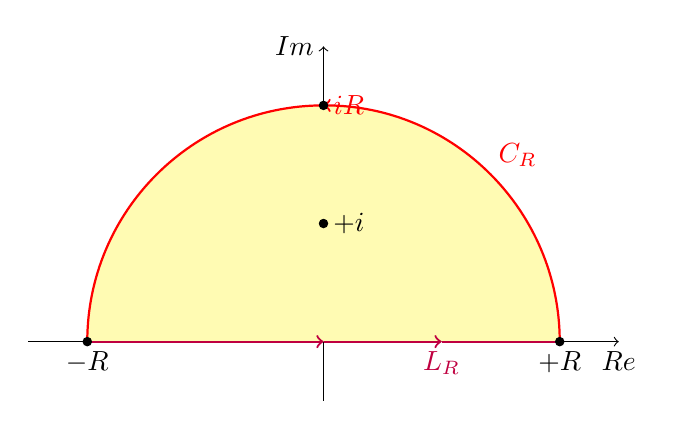
\begin{tikzpicture}[scale=1.5]
    % Axes
    \draw[->] (-2.5,0) -- (2.5,0) node[below] {$\operatorname{Re}$};
    \draw[->] (0,-0.5) -- (0,2.5) node[left] {$\operatorname{Im}$};
    
    % Contour
    \fill[yellow!30] (-2,0) arc (180:0:2) -- cycle;
    \draw[thick, red, ->] (2,0) arc (0:90:2);
    \draw[thick, red] (0,2) arc (90:180:2);
    \node[red, above right] at (1.4,1.4) {$C_R$};
    
    \draw[thick, purple, ->] (-2,0) -- (0,0);
    \draw[thick, purple, ->] (0,0) -- (1,0);
    \draw[thick, purple] (1,0) -- (2,0);
    \node[purple, below] at (1,0) {$L_R$};
    
    % Labels
    \filldraw (2,0) circle (1pt) node[below] {$+R$};
    \filldraw (-2,0) circle (1pt) node[below] {$-R$};
    \filldraw (0,2) circle (1pt) node[right, red] {$iR$};
    \filldraw (0,1) circle (1pt) node[right] {$+i$};
\end{tikzpicture}
\end{center}

Consider the closed curve $\gamma = L_R \cup C_R$ (boundary of the half-disc of radius $R$). The function $f(z) = \frac{1}{z^2+1} = \frac{1}{(z+i)(z-i)}$ has poles of order 1 at $\pm i$. 

From the residue theorem:
\[ \int_\gamma f(z) dz = 2\pi i \Res_i(f) \quad (\text{since } \interior(\gamma) \text{ contains only } i) \]
\[ \Res_i(f) = \lim_{z \to i} ((z-i)f(z)) = \lim_{z \to i} \frac{1}{z+i} = \frac{1}{2i} \]
So:
\begin{equation}
    \int_\gamma f(z) dz = \pi \label{eq:1}
\end{equation}

But, we also know:
\[ \int_\gamma f(z) dz = \int_{L_R} f(z) dz + \int_{C_R} f(z) dz \]
\begin{itemize}
    \item $\int_{L_R} f(z) dz = \int_{-R}^{R} \frac{1}{t^2+1} dt \xrightarrow{R \to +\infty} \int_{-\infty}^{+\infty} \frac{1}{x^2+1} dx$
    \item $\int_{C_R} f(z) dz = \int_{0}^{\pi} \frac{R \cdot i e^{it}}{1 + R^2 e^{2it}} dt$
\end{itemize}

We will show that $\int_{C_R} f(z) dz \xrightarrow{R \to +\infty} 0$.
\begin{align*}
    \left| \int_{C_R} f(z) dz \right| &= \left| \int_{0}^{\pi} \frac{R \cdot i e^{it}}{1 + R^2 e^{2it}} dt \right| \\
    &\le \int_{0}^{\pi} \frac{R \cdot |i e^{it}|}{|1 + R^2 e^{2it}|} dt
\end{align*}

Note: $|i e^{it}| = 1$ and, when $R \to +\infty$, $|1 + R^2 e^{2it}| \approx R^2$. 
Since, by the triangle inequality,
\[ |R^2 e^{2it}| - 1 \le |R^2 e^{2it} + 1| \le |R^2 e^{2it}| + 1 \]
We have $R^2 - 1 \le |1 + R^2 e^{2it}|$. Thus:
\[ \left| \int_{C_R} f(z) dz \right| \le \int_{0}^{\pi} \frac{R}{R^2 - 1} dt \approx \int_{0}^{\pi} \frac{R}{R^2} dt = \frac{\pi}{R} \xrightarrow{R \to +\infty} 0 \]

From \eqref{eq:1}, we deduce that:
\[ \int_{-\infty}^{+\infty} \frac{1}{1+x^2} dx = \pi \]
\end{example}